\documentclass[10pt]{article}
\usepackage[utf8]{inputenc}
\usepackage[paperwidth=16.3in,paperheight=7.2in,margin=0.2in]{geometry}
\usepackage{xcolor}
\usepackage{tikz}
\usetikzlibrary{arrows.meta,positioning}
\pagestyle{empty}
\pagecolor{white}

\begin{document}
\centering
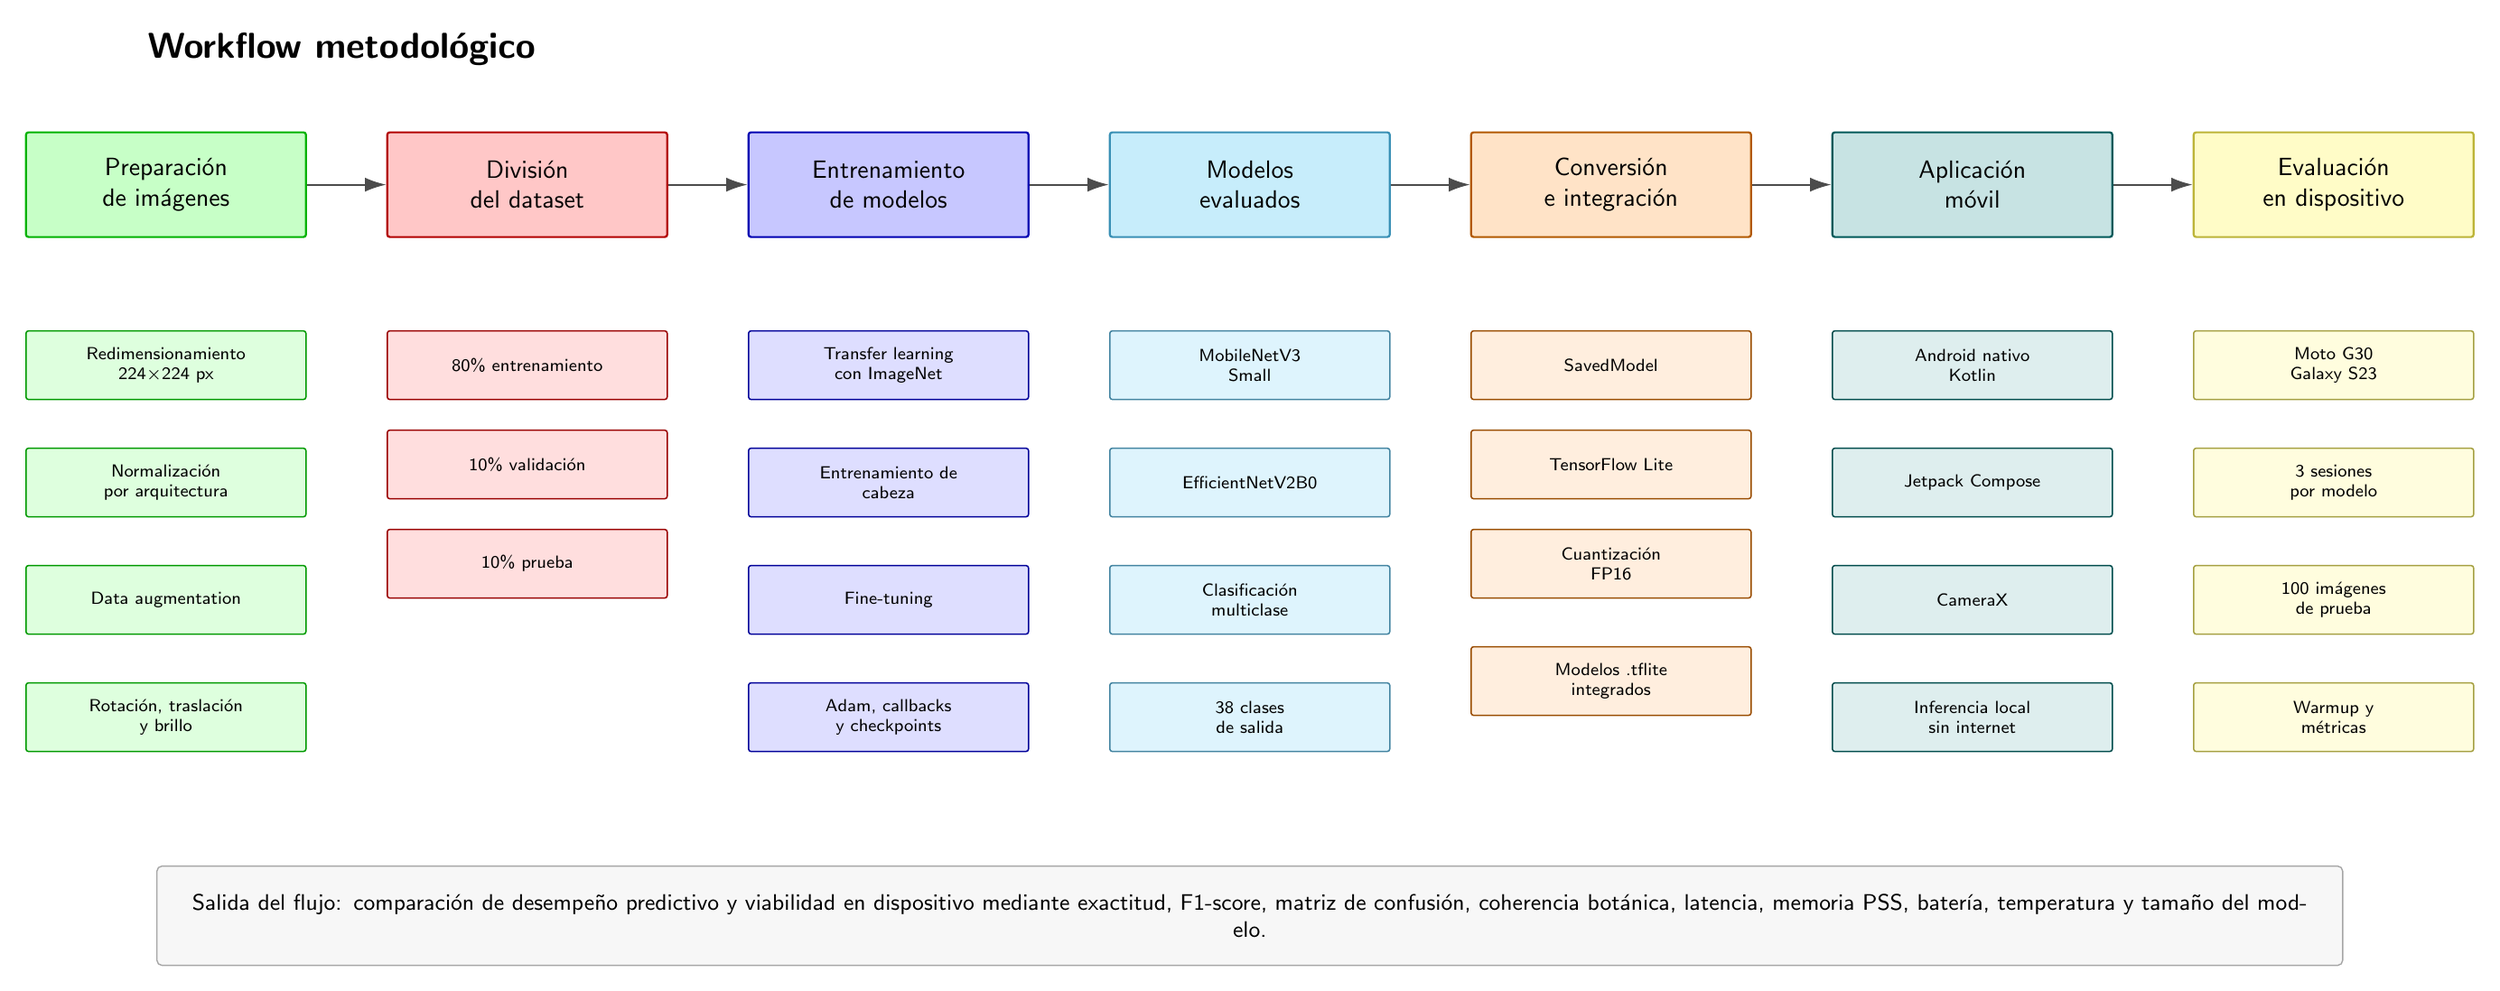
\begin{tikzpicture}[
    x=1in,
    y=1in,
    font=\sffamily,
    stage/.style={
        rectangle,
        draw=#1!70!black,
        fill=#1!22,
        line width=0.8pt,
        minimum width=1.55in,
        minimum height=0.58in,
        align=center,
        rounded corners=1pt
    },
    item/.style={
        rectangle,
        draw=#1!60!black,
        fill=#1!13,
        line width=0.55pt,
        minimum width=1.55in,
        minimum height=0.38in,
        align=center,
        rounded corners=1pt,
        font=\sffamily\scriptsize
    },
    flowarrow/.style={-{Latex[length=3mm,width=2mm]}, line width=0.7pt, draw=black!70}
]

\node[font=\sffamily\bfseries\Large, anchor=west] at (-0.15, 0.75) {Workflow metodológico};

\node[stage=green] (s1) at (0,0) {Preparación\\de imágenes};
\node[stage=red] (s2) at (2.0,0) {División\\del dataset};
\node[stage=blue] (s3) at (4.0,0) {Entrenamiento\\de modelos};
\node[stage=cyan] (s4) at (6.0,0) {Modelos\\evaluados};
\node[stage=orange] (s5) at (8.0,0) {Conversión\\e integración};
\node[stage=teal] (s6) at (10.0,0) {Aplicación\\móvil};
\node[stage=yellow] (s7) at (12.0,0) {Evaluación\\en dispositivo};

\foreach \a/\b in {s1/s2,s2/s3,s3/s4,s4/s5,s5/s6,s6/s7}
    \draw[flowarrow] (\a.east) -- (\b.west);

\node[item=green] at (0,-1.0) {Redimensionamiento\\224$\times$224 px};
\node[item=green] at (0,-1.65) {Normalización\\por arquitectura};
\node[item=green] at (0,-2.30) {Data augmentation};
\node[item=green] at (0,-2.95) {Rotación, traslación\\y brillo};

\node[item=red] at (2.0,-1.0) {80\% entrenamiento};
\node[item=red] at (2.0,-1.55) {10\% validación};
\node[item=red] at (2.0,-2.10) {10\% prueba};

\node[item=blue] at (4.0,-1.0) {Transfer learning\\con ImageNet};
\node[item=blue] at (4.0,-1.65) {Entrenamiento de\\cabeza};
\node[item=blue] at (4.0,-2.30) {Fine-tuning};
\node[item=blue] at (4.0,-2.95) {Adam, callbacks\\y checkpoints};

\node[item=cyan] at (6.0,-1.0) {MobileNetV3\\Small};
\node[item=cyan] at (6.0,-1.65) {EfficientNetV2B0};
\node[item=cyan] at (6.0,-2.30) {Clasificación\\multiclase};
\node[item=cyan] at (6.0,-2.95) {38 clases\\de salida};

\node[item=orange] at (8.0,-1.0) {SavedModel};
\node[item=orange] at (8.0,-1.55) {TensorFlow Lite};
\node[item=orange] at (8.0,-2.10) {Cuantización\\FP16};
\node[item=orange] at (8.0,-2.75) {Modelos .tflite\\integrados};

\node[item=teal] at (10.0,-1.0) {Android nativo\\Kotlin};
\node[item=teal] at (10.0,-1.65) {Jetpack Compose};
\node[item=teal] at (10.0,-2.30) {CameraX};
\node[item=teal] at (10.0,-2.95) {Inferencia local\\sin internet};

\node[item=yellow] at (12.0,-1.0) {Moto G30\\Galaxy S23};
\node[item=yellow] at (12.0,-1.65) {3 sesiones\\por modelo};
\node[item=yellow] at (12.0,-2.30) {100 imágenes\\de prueba};
\node[item=yellow] at (12.0,-2.95) {Warmup y\\métricas};

\node[draw=black!35, fill=black!3, rounded corners=2pt, line width=0.5pt, align=center,
      minimum width=12.1in, text width=11.8in, minimum height=0.55in, font=\sffamily\small] at (6.0,-4.05)
      {Salida del flujo: comparación de desempeño predictivo y viabilidad en dispositivo mediante exactitud, F1-score,
      matriz de confusión, coherencia botánica, latencia, memoria PSS, batería, temperatura y tamaño del modelo.};

\end{tikzpicture}
\end{document}
